\documentclass[a4paper,11pt]{article}

\usepackage{graphicx}

\title{Comparison of language execution times}
\author{Pete Sanders  \\
	Home Project
	}

\date{\today}

\begin{document}

\maketitle

\tableofcontents

\section{Introduction}

\section{Languages}

\subsection{Language differences}

\section{Use cases}

The purpose of the use-cases is to have a realistic blend of arithmatic (integer and floating-point), logic, 
comparisons, program flow and memory operations. Though each use-case will have a different ratio of these features.

The use-cases are algorithms taken from the realms of mathematics and computer science.
Each is a self contained solution to a problem which uses general-purpose features 
of the language they are written in. Each use-case is written in an easy-to-understand way
and are not heavily optimised. 
The use-cases are written the same in each language, unless the language does not allow.

The output of each use-case is a short text file which guarentees the correctness. 

\subsection{Pythagorean triples}
\subsection{Linear congruential number generator}
\subsection{XOR shift number generator}
\subsection{Fibonacci series}
\subsection{Kaprekars process}
\subsection{Naughts and crosses}
\subsection{Triangle enclosure}
\subsection{Unique anagram}
\subsection{Goldbach conjecture}
\subsection{Sieve of Eratosthenes}
\subsection{Pi from random numbers}

\section{Results}

\subsection{Platforms}

\begin{center}
 \begin{tabular}{|| c | c | c ||} 
\hline 
Short Name & Attribute & Version Information  \\ 
 \hline
Sony Vaio  \footnote{Windows information retrieved with 'systeminfo',  'wmic cpu get' and 'wmic memorychip get'}
& Make/Model
& Sony Corporation\\
& &  Vaio VPCEH2P0E \\
\cline{2-3}
& CPU
& Intel64 Family 6 Model 42 Stepping 7 \\
& & Intel(R) Core(TM) i5-2430M CPU @ 2.40GHz \\
& & 2 cores \\
\cline{2-3}
&  RAM
& 2 x 4GB DDR3 SODIMM \\
& & 64bit width,?? MHz\\ 
\cline{2-3}
& OS
& Microsoft Windows 10 Home\\
& & 10.0.18363 N/A Build 18363 \\
 \hline \hline
\end{tabular}
\end{center}


\subsection{Language details}

\begin{center}
\begin{tabular}{|| c | c | c ||} 
\hline 
Short Name & Language & Version Information  \\ 
\hline
Sony Vaio
& C/gcc
& MinGW cc.exe (GCC) 4.6.2 \\
& & 2011 Free Software Foundation, Inc.\\
\cline{2-3}
& C/MSVC
& Microsoft (R) C/C++ Optimizing Compiler \\
& & Version 19.25.28614 for x64 \\
\cline{2-3}
&  Go
& go version go1.11.2 windows/amd64 \\
\cline{2-3}
& Java
& javac 1.7.0\_60-ea \\ 
& & java version "1.8.0\_161" \\ 
& & Java(TM) SE Runtime Environment (build 1.8.0\_161-b12) \\
\cline{2-3}
& Python
& Python 3.6.9 (2ad108f17bdb, Apr 07 2020, 03:05:35) \\
& & [PyPy 7.3.1 with MSC v.1912 32 bit] \\
 \hline \hline
\end{tabular}
\end{center}


\subsection{Timings}

\begin{figure}[h]
\centering
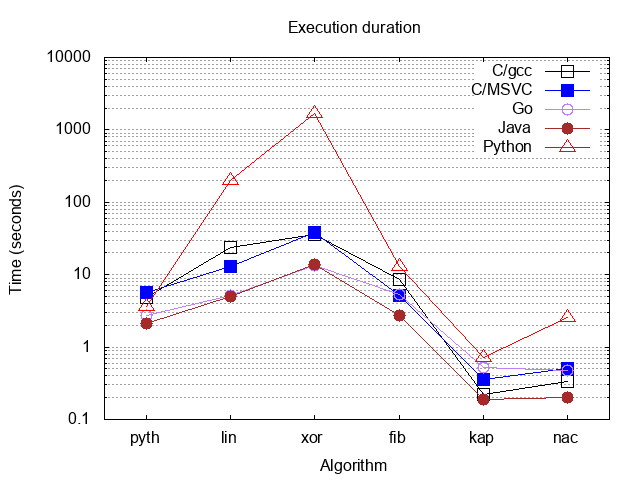
\includegraphics[scale=0.75]{"v1/times.png"}
\end{figure}

\begin{figure}[h]
\centering
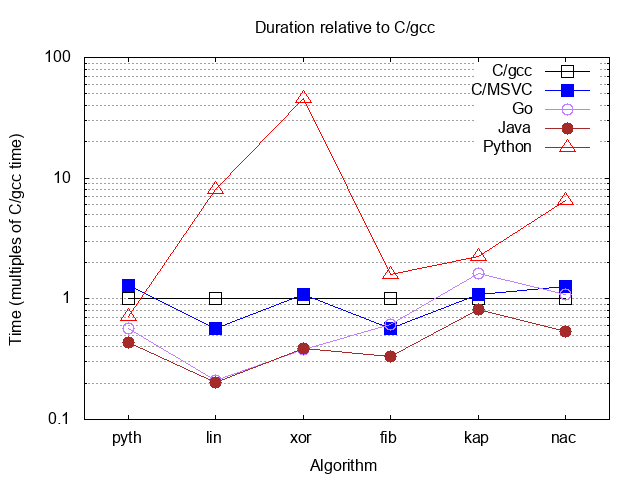
\includegraphics[scale=0.75]{"v1/normalised.png"}
\end{figure}

\end{document}
